\chapter{User Guide}
\label{ch:user_guide}

In the previous chapters we developed and evaluated several methods for a known-item-search task. In this chapter we provide a user guide for our implementation of aforementioned solutions. This chapter only covers user interaction and does not cover expreimenting with new datasets nor overview of the implementation.

The user can access the application via web-based interface. Once the webpage is opened we can see by default a module for search based on the collage (refer to \ref{ch:object_location}). The second module includes face similarity search (chapter \ref{ch:face_search}). We describe both modules in the same order.

\section{Running the application}

The easiest way to run the application is to install Docker\footnote{\url{https://docs.docker.com/desktop/}}. Once the Docker is installed, it is enough to run following commands from the top level directory, i.e., where \verb+README.md+ is located.

\vspace{0.5cm}

\begin{boxedverbatim}
# ./thesis-grizzly/
$ docker build . -t app
$ docker run -p 8000:8000  \
  -v $PWD/image_representations:\
      /diplomova_praca/static/image_representations \
  -t app
\end{boxedverbatim}

\vspace{0.5cm}

Once the application is running, you can access the it via browser (tested on Google Chrome version 84.0.4147.89) at following url adress: \url{http://127.0.0.1:8000/}. The first initialization takes longer, the website will load itself once it has started. 

\subsection*{Included dataset}

The provided demo includes a dataset of images to search on. These images come from Open Image Dataset\footnote{\url{https://opensource.google/projects/open-images-dataset}, CC-by 4.0}. The dataset contains 20\,035 images, for which we computed the region splitting for 2x4 regions. For an approach using antepenultimate layer, we only provide extracted features for half of the dataset, due to the size limit of attachments. Finally, we extracted 528 faces from the dataset, which are used for the search by collage (with the same settings as described in \autoref{ch:face_search}).

The data, which the model uses is by default in the directory \verb+image_representation+. In the next chapter we describe how to obtain the data, it is possible to either replace the existing or to create a new directory and update the path in the provided example.

\section{Modules}

Our application is separated to two modules: spatial search and face search. User can switch between the modules in the top right corner. Now we shortly describe a typical interaction of the user with the system for each module.

\subsection{Search by Collage}

The default module, which opens, is search by collage. On the screen we can see a canvas for creating the queries and some control elements. On the first load, a target image (the searched scene) is displayed for several seconds over the canvas. During the creation of the collage we can always access the target image by clicking on the image button (``Display hint''), check the \autoref{fig:ui_collage}.

\subsubsection*{Creating a collage}

We can create custom collages in the canvas. In order to add an image to the canvas, we can either \emph{paste} it, or add it based on the url of the image. To paste an image, it needs to be available in the clipboard. The easiest way to do that for most images is to right click on the image and select ``Copy image''. We can also recommend a selective screenshot features, which can speed up the copying of the images and also add possibility for selecting only a part of the image. For Windows 10 it is possible via key combination Shift + Win Key + S. 

There is no limitation on the number of images in the collage, although the increased number may reduce the performance (as they may be misleading hints) in recall and also it prolongs the computation time needed for the query to process.

Once the image is placed in the canvas, we can resize it by grabbing bottom right corner, or move it by dragging. To remove the image click on the \verb+x+ button in the top right corner. To query the model, click the ``Query'' button. By default, automatic querying is turned on, i.e., after each movement or resizing the system automatically query the dataset. This can be turned off, which comes handy, if the model with longer inference time is used.

It is possible to switch between the approaches used  for feature extraction. The list of available approaches can by accessed by clicking on the three dots, next to the query button.

\subsubsection*{Displayed results}

\begin{figure}
    % \centering
    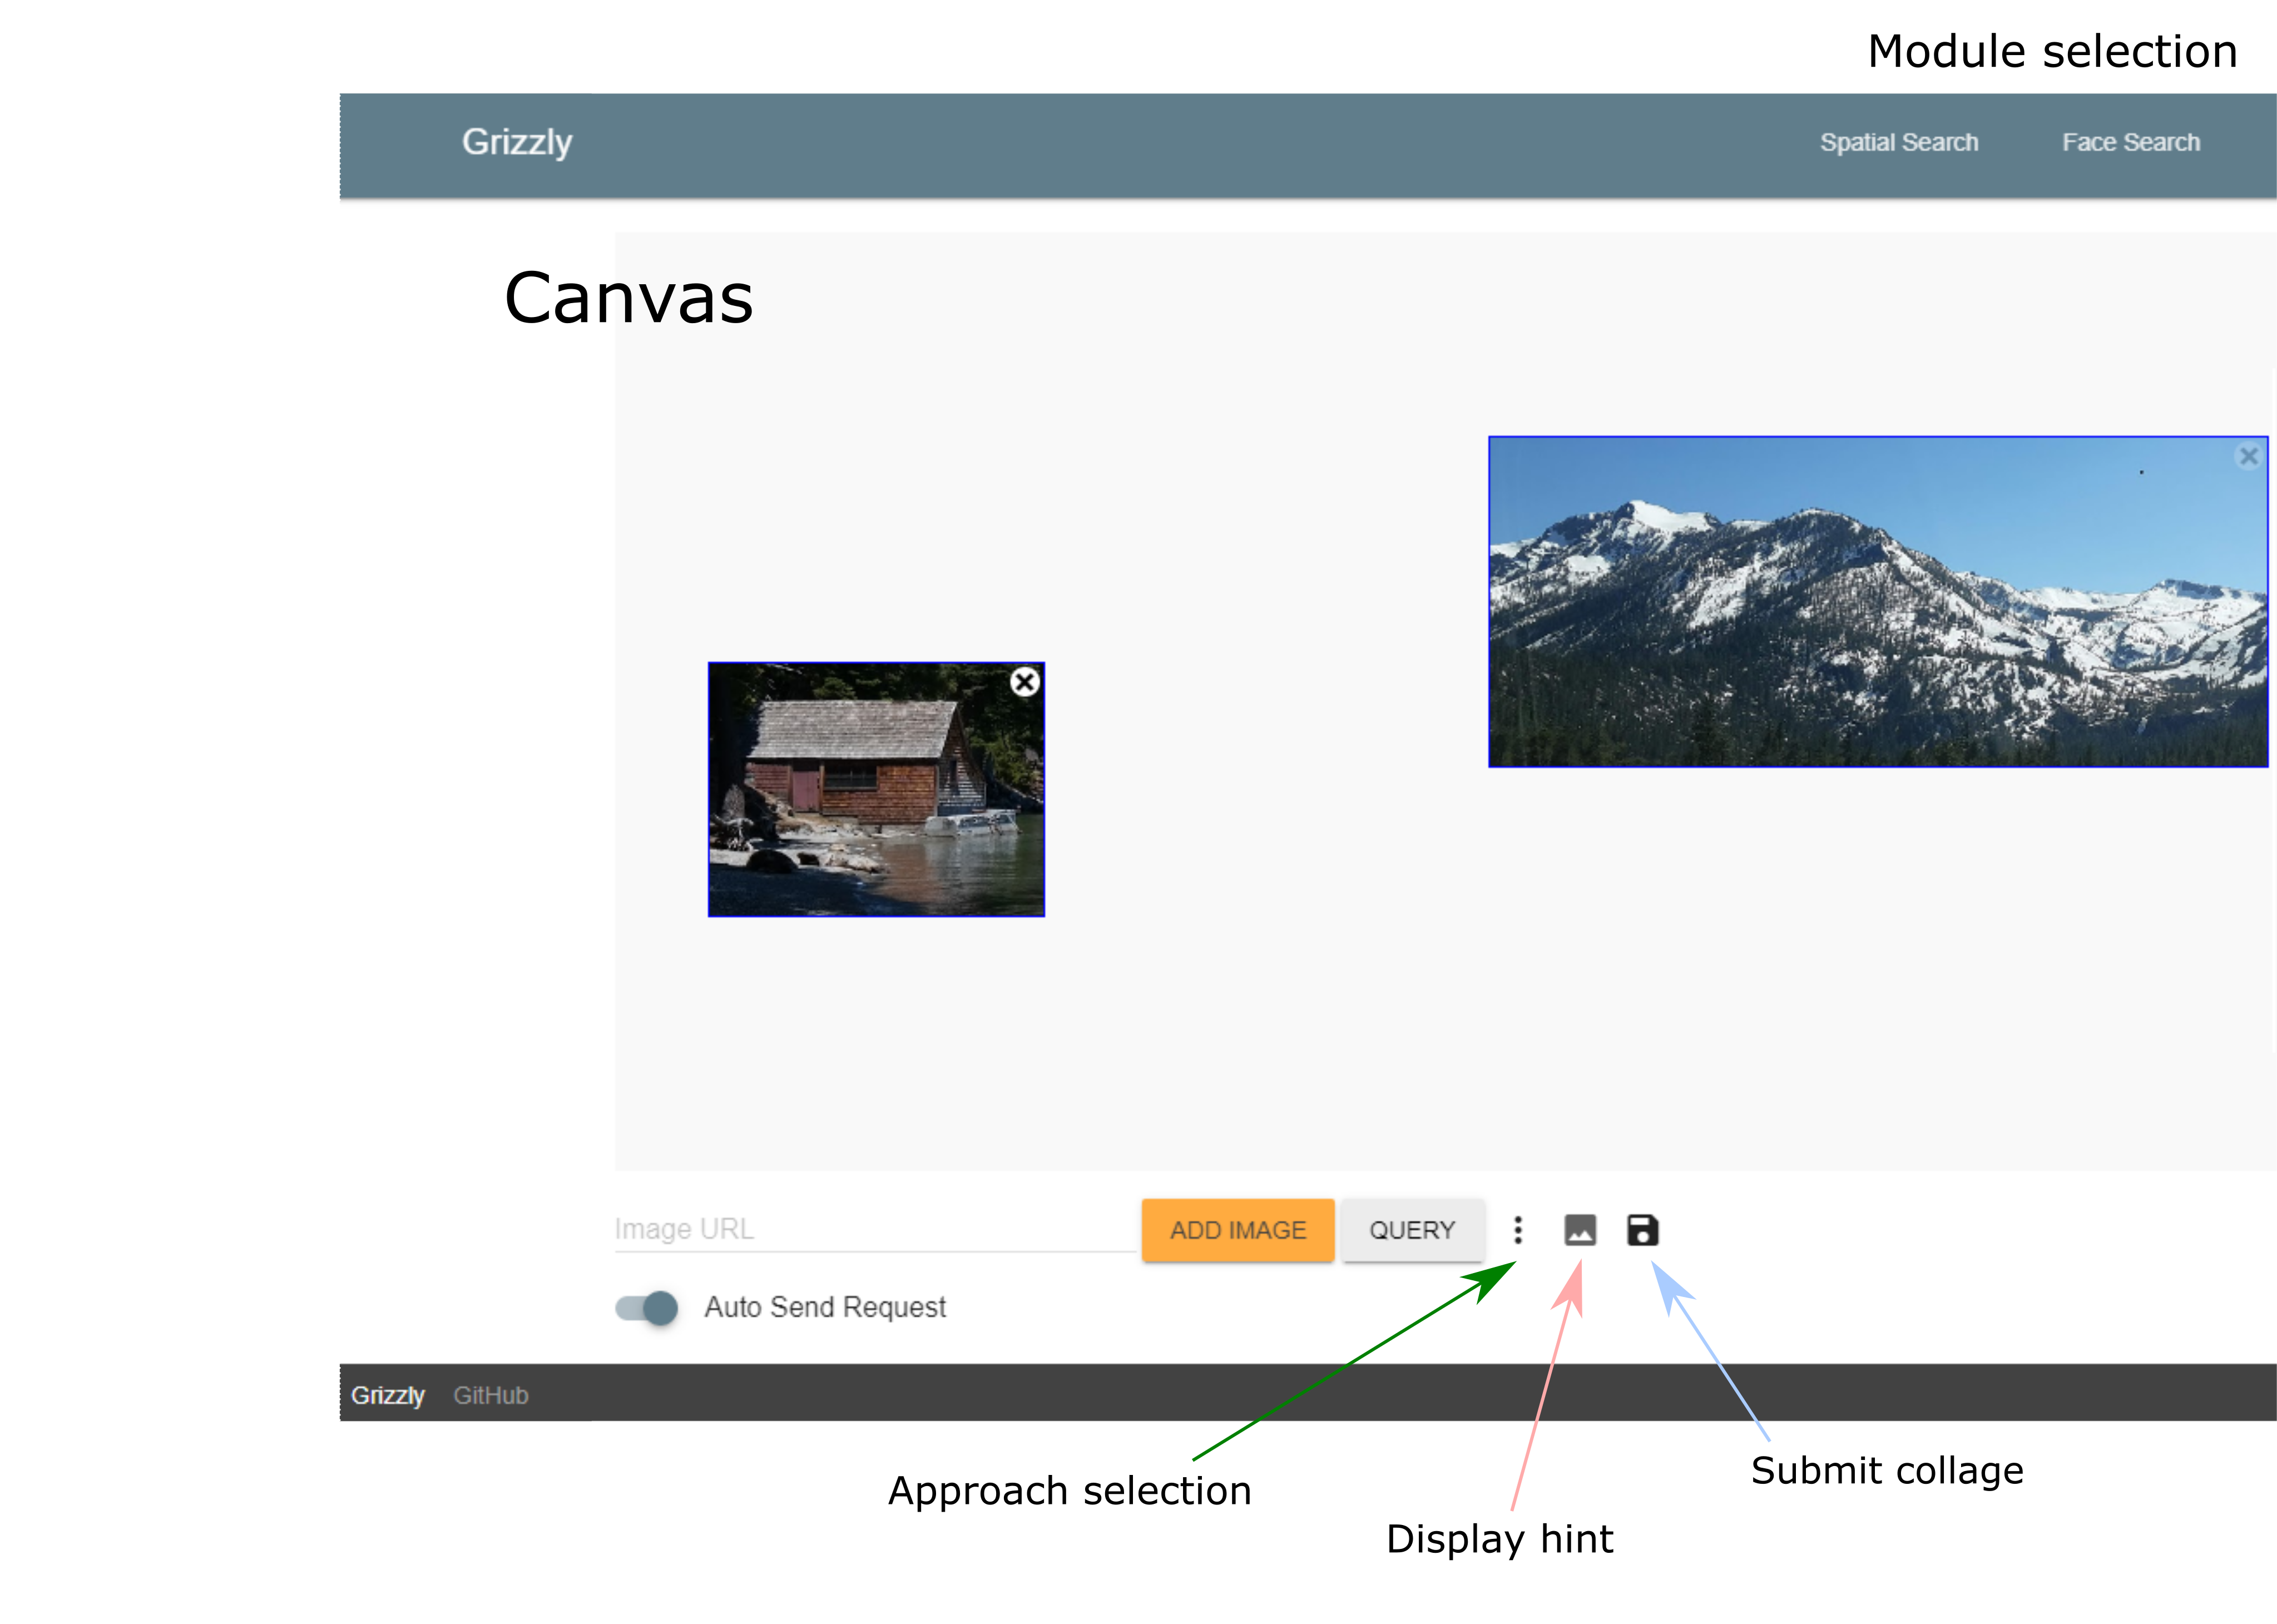
\includegraphics[width=0.9\linewidth]{img/spatial_ui.png}
    \caption{User interface for creating collages}
    \label{fig:ui_collage}
\end{figure}

By default, the application displays only the best 100 matched results. The images are reloaded after each successful query. The top of the Results section also displays the rank of the searched item. This helps for the user to learn how to use the tool more effectively. The winning regions are highlighted as well for the regions search by orange rectangle.

Results are presented based on the ranking, as we described in \autoref{s:task_formulation}. More similar results are displayed first. If the image is not present in loaded dataset, the rank will not be displayed. This may be a case, where the features for a given approach are not available for all images in the dataset.

\subsection{Search by face similarity}

\begin{figure}
    \centering
    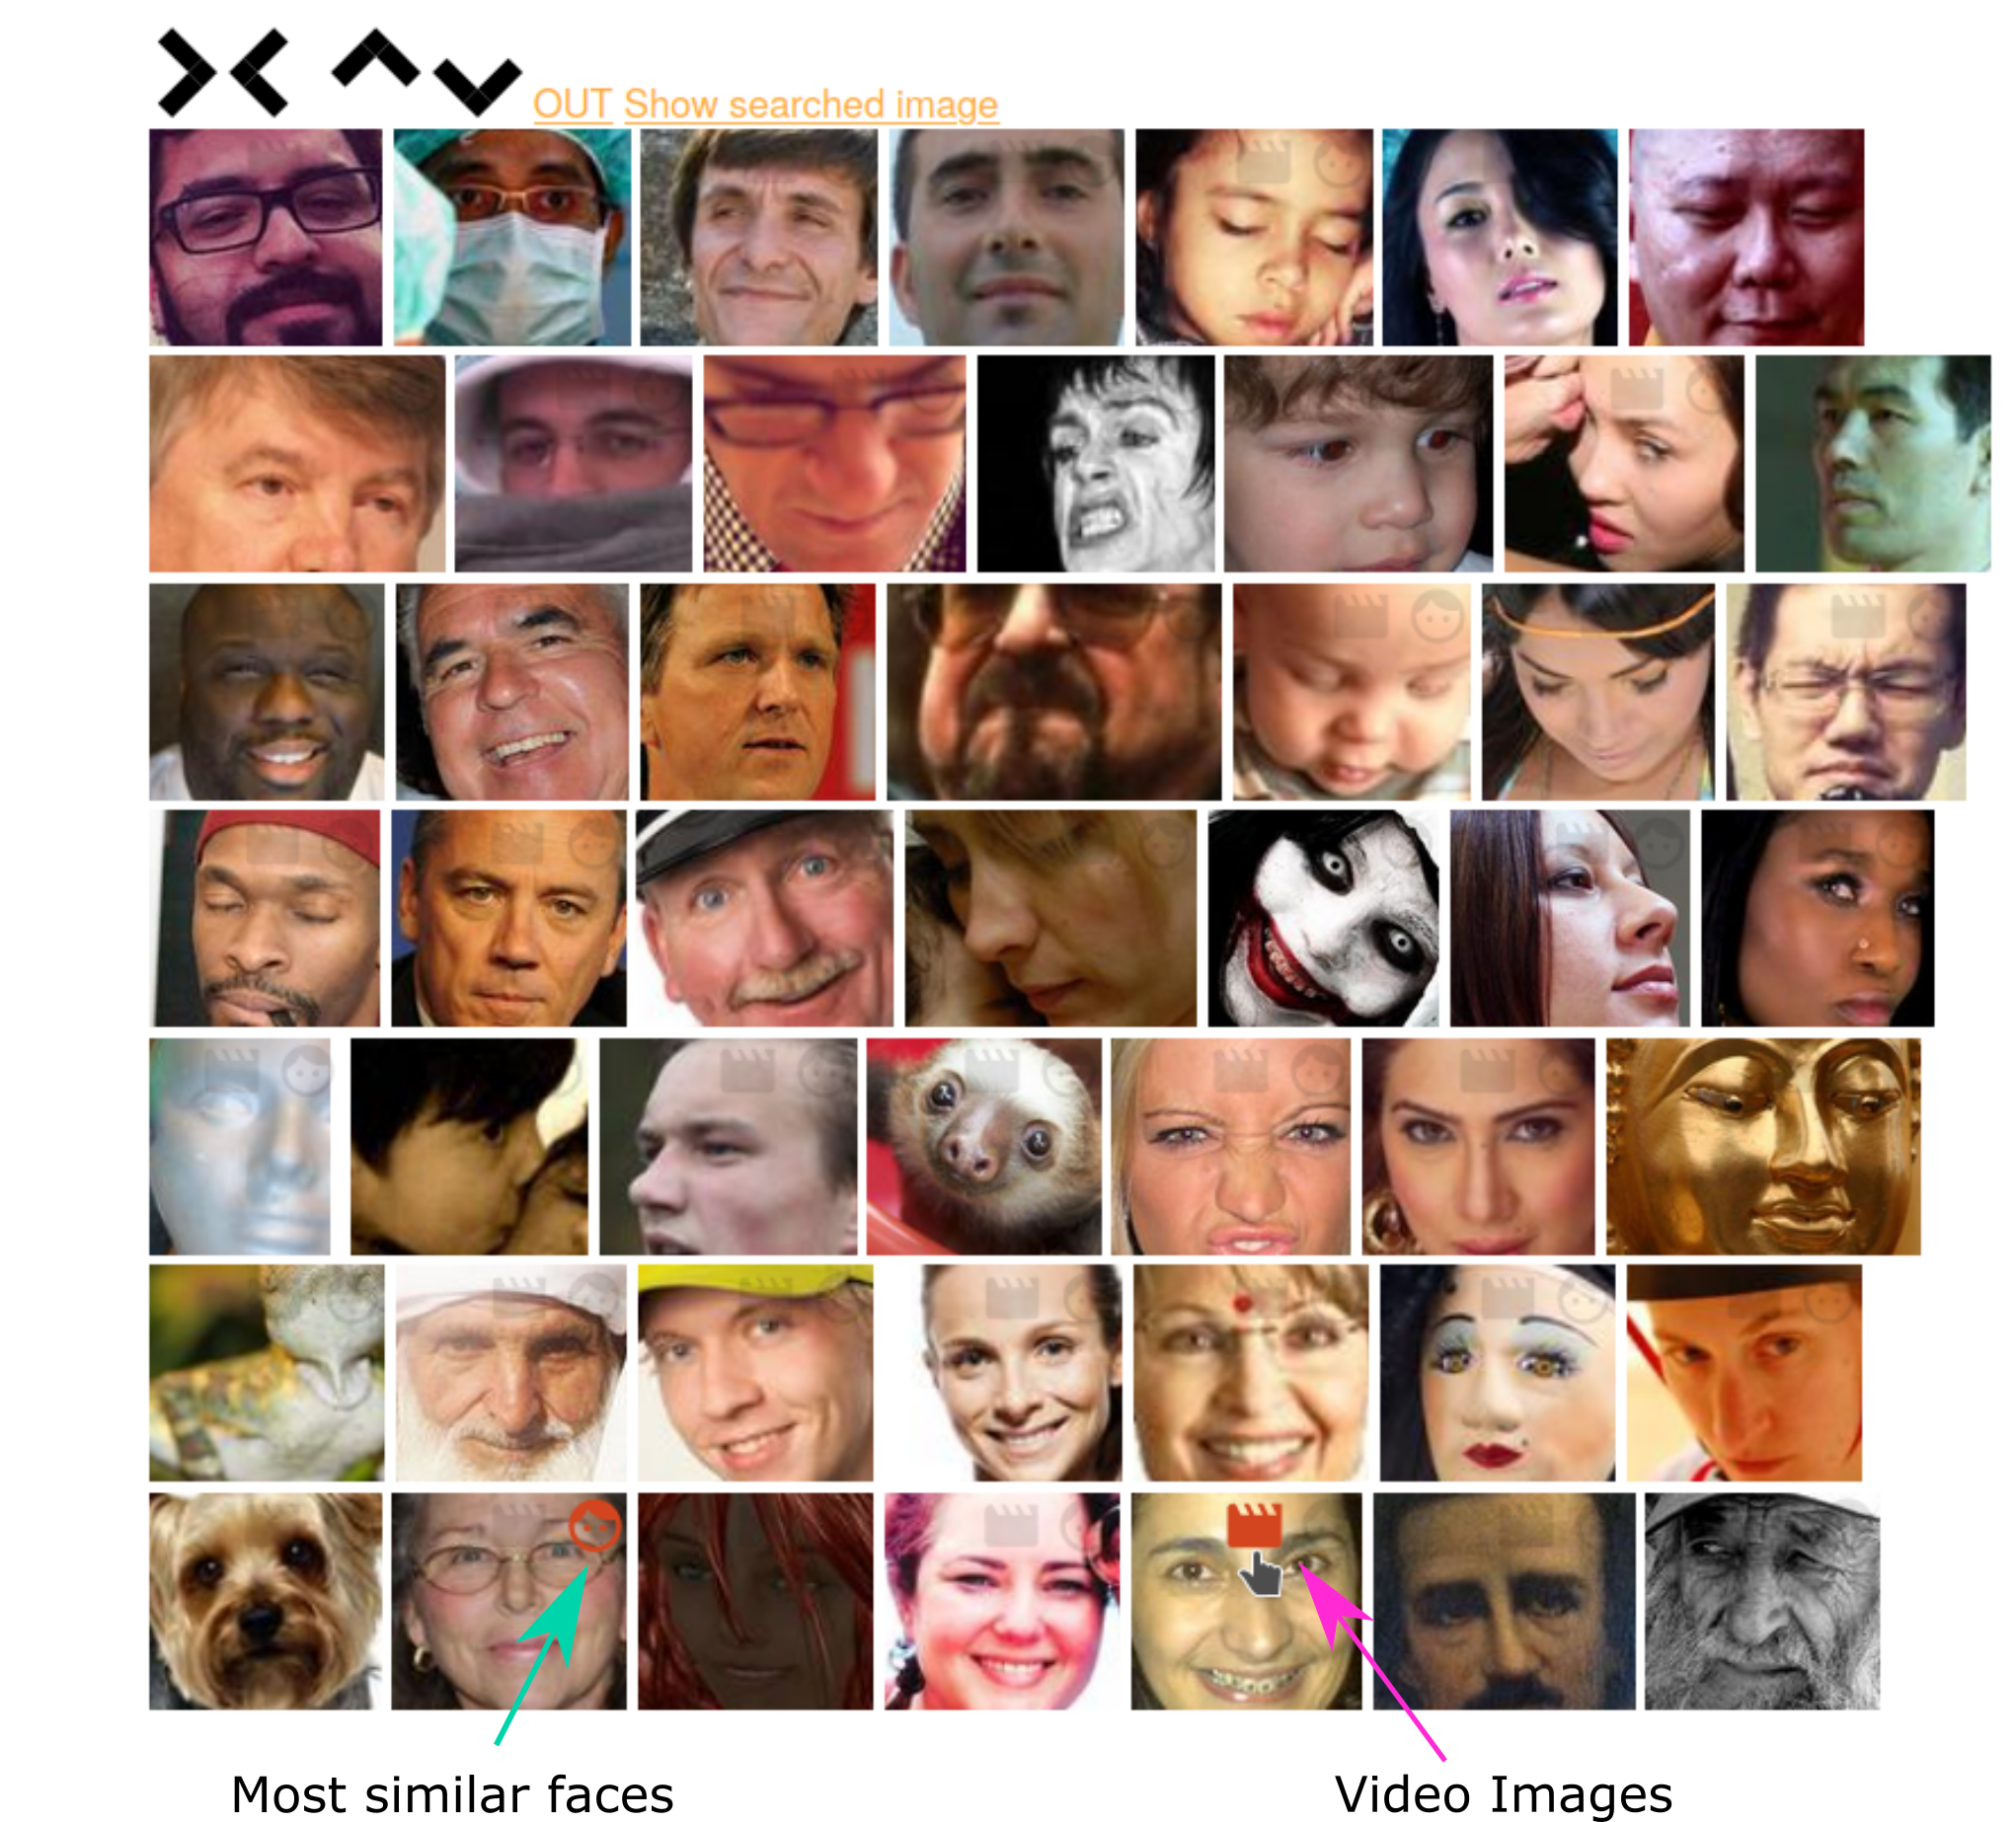
\includegraphics[width=\linewidth]{img/face_grid.png}
    \caption{Top layer of our traversal structure.}
    \label{fig:face_grid_app}
\end{figure}

Upon loading the face module, there is a grid. with faces and also a target image is displayed. Similarly to the Search by collage module, the target image can be accessed at any moment by clicking on \verb+Show the image+. 

The grid, which is displayed represents the top layer of the multilevel structure. This layer fully fits into a display, therefore, move commands do not have an effect. We can step up from any (except top layer, where it does not have any effect) layer by clicking on link \verb+Out+.

By clicking at any face, we step down one layer. The image which we clicked is in the center of the next layer, if possible. This is not possible for images near the corners, therefore, it is displayed in a way, that full display is used, and is as close as possible to the center.

Each image in the traversal structure also supports two additional operations: show images from the video and show closest faces. In case of images, which did not come from the videos (the case of the demo dataset), the images displayed by it are arbitrary. The second option displays all images, which contain a face similar to the queried. Both these options are available by corresponding icons in the top right corner of the face, available at any layer. A top layer for our demo dataset is displayed in the figure \ref{fig:face_grid_app}










\chapter{Extracting features for new datasets}

In the previous chapter, we described how to run a demo with preprocessed dataset of images. In this chapter we describe steps required to run the application for a new set of images. In case, the images do not change, only a single approach (i.e., using a different network), it is enough to do only the corresponding step.

Our feature extraction is a two step process. We again use docker, to avoid dependency problems. The extraction process belongs to our separate module -- \verb+diplomova_praca_lib+. Therefore,we  firstly change the working directory and then we build a single docker container, which we use for all extractions.

\vspace{0.5cm}
\begin{boxedverbatim}
$ cd diplomova_praca_lib
$ docker build . -t lib
\end{boxedverbatim}
\vspace{0.5cm}

Images we use for the extraction should by separated by the videos by directory structure. If the images do not have any temporal context, it is possible to split them to different directories, or to create one directory with all images.

\section{Feature extraction for Collage approaches}

In this section we provide an example of extracting features for our system for both collage approaches: regions and using the last convolution block. In this example, we extract features by \verb+MobileNetV2+, using regions \verb+2x4+ with the \verb+input_size=96+. The system expects equally sized images.

\vspace{0.5cm}
\begin{boxedverbatim}
$ images="/path/to/images/"
$ intermediate_output="/path/to/intermediate_output/"
$ features="/path/to/features/"

$ docker run \
  -v $images:/images \
  -v $intermediate_output:/feature_records \
  lib \
   python diplomova_praca_lib/annotate_images.py \
    --images_dir=/images --save_location=/feature_records \
    --feature_model=mobilenetv2 --num_regions=2,4 \
    --input_size=96

$ docker run \
  -v $intermediate_output:/feature_records \
  -v $features:/features \
  lib \
    python diplomova_praca_lib/preprocess_data.py \
      --input=/feature_records --output=/features 
      --transform --regions --explained_ratio=128
\end{boxedverbatim}

\vspace{0.5cm}

Parameters options for feature extraction:
\begin{itemize}
    \item \verb+--feature_model+:\verb+resnet50v2+, \verb+resnet50v2antepenultimate+, \verb+mobilenetv2+, \verb+mobilenetv2antepenultimate+.
    \item \verb+--input_size+: depends on the model used, check with Keras Applications
    \item \verb+--num_regions+: other values evaluated in this thesis were 2x3, 3x5. Other viable options are allowed.
\end{itemize}

The second step includes preprocessing with optional PCA dimension reduction. The parameters are:
\begin{itemize}
    \item \verb+--empty_pipeline+: no PCA is applied, data are only preprocessed forming structure for the application or
    \item \verb+--explained_ratio=128+: PCA into given number of components is applied
    \item \verb+--regions+: to specify that the data reflect the regions' structure
\end{itemize}

The content of the \verb+$features+ can be than copied to the corresponding directory and immediately used.

\section{Feature extraction for Face Similarity}

For the extraction of faces and their encodings, we use similar steps as in the previous section:

\vspace{0.5cm}
\begin{boxedverbatim}
$ images="/path/to/images/"
$ intermediate_output="/path/to/intermediate_output/"
$ features="/path/to/features/"

$ docker run \
  -v $images:/images \
  -v $intermediate_output:/feature_records \
  lib \
   python diplomova_praca_lib/annotate_images.py \
    --images_dir=/images --save_location=/feature_records \
    --feature_model=faces

$ docker run \
  -v $intermediate_output:/feature_records \
  -v $features:/features \
  lib \
    python diplomova_praca_lib/preprocess_face_data.py \
      --input=/feature_records --output=/features \
      --crop_size=0.08
\end{boxedverbatim}
\vspace{0.5cm}

where the \verb+crop_size+ specifies filtering criteria on the minimum area covered by the face in the image.

\subsection{Training Self-organizing map}

After obtaining the face encodings, we can train the underlying self-organizing map, which we use to obtain a grid of faces for the bottom layer.


\vspace{0.5cm}
\begin{boxedverbatim}
$ face_features="/path/to/face_features/"
$ trained_som="/path/to/trained_som/"

$ docker run \
  -v $face_features:/features \
  -v $trained_som:/output \
  lib \
   python diplomova_praca_lib/train_som.py \
    --input=/features \
    --iterations=200000
\end{boxedverbatim}
\vspace{0.5cm}

For \verb+train_som.py+ additional arguments as \verb+learning_rate+, \verb+sigma+, \verb+distance+ may be explored. The scripts saves all intermediate self-organizing maps and also plots the errors during the training. It is possible to choose any of those for the application and observe the differences between them.

\section{Running the server with new data}

By the new data we can replace any of the existing ones, either in their original location \verb+images_representations+, or we can create a new location for the data with following structure:


\vspace{0.5cm}
\begin{boxedverbatim}
image_representations/
    faces/
        features/
            faces.npz
        som/
            som.pickle
    images/
        000/
            image1.jpg
        001/
            image2.jpg
    regions/
        model-mobilenetv2,dir=000.npz
        model-mobilenetv2,dir=001.npz
    spatial/
        model-mobilenetv2antepenultimate,dir=000.npz
        model-mobilenetv2antepenultimate,dir=001.npz
\end{boxedverbatim}
\vspace{0.5cm}

It is not necessary to provide all data for all approaches. Only the modules with correctly provided data will work as expected.






























\chapter{Implementation Overview}
\label{ch:developers_guide}
\label{ch:programmers_guide}

Our implementation covers a wide range of topics. This thesis required a fullstack implementation -- from creating a web-based frontend to library able to work with machine learning models. Therefore, we do not include an exhaustive enumeration of the modules, and steps required, but we provide an overview of the whole approach in figure \ref{}.

This figure represents the individual layers of our solution, naming the technologies used in our solution. For more details, we refer to the individual modules in our code. At last, we would like to appreciate all used frameworks, especially Scikit-learn \citep{pedregosa2011scikit} and NumPy \citep{van2011numpy}.


% In this chapter we provide an overview

% \section{Code Overview}
% To provide a brief, structured overview of the project, we firstly provide an overview of used libraries and frameworks. We continue by describing the modules of our application.

% Our application is split into two parts: web-based application and the library. In the web application, we include the frontend for creating queries and interactive environment for the search. In the library, we perform every part of the inference.

% \subsection{Libraries and Frameworks}

% Our language of choice is mainly Python (v3.7). We selected this languages due to its popularity among the machine learning community. Based on this choice, we wanted to limit the number of programming languages used in this project. We therefore select Django, as our choice for web framework.  We further describe both individually.

% \subsubsection{Web-based application}

% For ourproject we chose Django (v3.0.8) as our web-framework. For interactive frontend we further use JavaScript to implement features like rescaling, dragging, etc.

% \subsubsection*{CSS}

% We use Syntactically Awesome Style Sheets\footnote{\url{https://sass-lang.com/}} (SCSS) to generate our CSS files. This provides us with an advantage to use variables and nesting to reduce the size and repetition of our CSS files.

% \subsubsection*{JavaScript}

% We use pure JavaScript in combination with jQuery\footnote{\url{https://jquery.com/}} to power our web interface. Regarding the querying process from our frontend to the Django, we use mostly AJAX requests (asynchronous HTTP). We use \verb+POST+ method to send the data to Django, which we encode into string using JSON.

% \subsubsection*{Material Design Lite\footnote{\url{https://getmdl.io/}}}

% For the frontend we use Material Design Lite. In our application we use several components from the Material Design Lite, including: buttons, icons, layouts, loading and other.

% \subsubsection{Library}

% \cite{pedregosa2011scikit}
% \cite{van2011numpy}

